% =====================================================================
% BMED365 (Spring 2027) — Lab 4: Kiwi 7T MRI Seed Segmentation Challenge
% Companion Guide: Frontier Biomedical AI Paradigms on 7T MRI
% Compile with: pdflatex frontier-ai-paradigms.tex (run twice)
% =====================================================================
\documentclass[10.5pt,a4paper]{article}

\usepackage[utf8]{inputenc}
\usepackage[T1]{fontenc}
\usepackage[english]{babel}
\usepackage{lmodern}
\usepackage{microtype}
\usepackage{graphicx}
\usepackage{booktabs}
\usepackage{tabularx}
\usepackage{array}
\usepackage{colortbl}
\usepackage{xcolor}
\usepackage{amsmath,amssymb}
\usepackage{enumitem}
\usepackage[margin=1.9cm,headheight=14pt]{geometry}
\usepackage{fancyhdr}
\usepackage{titlesec}
\usepackage[most]{tcolorbox}
\usepackage{listings}
\usepackage{float}
\usepackage{tikz}
\usetikzlibrary{arrows.meta,positioning,shapes.geometric,fit,backgrounds,calc}
\usepackage{hyperref}

% =====================================================================
% COLORS & HYPERREF (UiB / BMED365 House Style)
% =====================================================================
\definecolor{uibblue}{RGB}{0, 61, 115}
\definecolor{uibred}{RGB}{175, 28, 44}
\definecolor{kiwigreen}{RGB}{27, 138, 90}
\definecolor{amberwarn}{RGB}{195, 110, 0}
\definecolor{lightgray}{RGB}{246, 248, 250}
\definecolor{rowalt}{RGB}{242, 246, 251}
\definecolor{codebg}{RGB}{248, 249, 251}
\definecolor{codekw}{RGB}{0, 75, 145}
\definecolor{codestr}{RGB}{155, 35, 45}
\definecolor{codecmt}{RGB}{95, 105, 115}

\hypersetup{
    colorlinks=true,
    linkcolor=uibblue,
    citecolor=uibblue,
    urlcolor=uibred,
    pdftitle={Frontier Biomedical AI Paradigms on the 7T MRI Kiwi Challenge (BMED365 Spring 2027)},
    pdfauthor={Arvid Lundervold (UiB / MMIV) -- BMED365 Spring 2027}
}

% =====================================================================
% TYPOGRAPHY, HEADERS & CALLOUT BOXES
% =====================================================================
\setlength{\parindent}{0pt}
\setlength{\parskip}{0.45em}
\setlist[itemize]{topsep=2pt,itemsep=2pt,leftmargin=1.4em}
\setlist[enumerate]{topsep=2pt,itemsep=2pt,leftmargin=1.6em}

\newcolumntype{L}[1]{>{\raggedright\arraybackslash}p{#1}}
\newcolumntype{C}[1]{>{\centering\arraybackslash}p{#1}}
\newcolumntype{R}[1]{>{\raggedleft\arraybackslash}p{#1}}
\newcolumntype{Y}{>{\raggedright\arraybackslash}X}

\titleformat{\section}{\Large\bfseries\color{uibblue}}{\thesection}{0.7em}{}[\vspace{1pt}\titlerule]
\titleformat{\subsection}{\large\bfseries\color{uibblue!88!black}}{\thesubsection}{0.6em}{}
\titleformat{\subsubsection}{\normalsize\bfseries\color{uibblue!75!black}}{\thesubsubsection}{0.5em}{}
\titlespacing*{\section}{0pt}{1.15em}{0.45em}
\titlespacing*{\subsection}{0pt}{0.85em}{0.3em}

\pagestyle{fancy}
\fancyhf{}
\fancyhead[L]{\footnotesize\textcolor{gray}{BMED365 (Spring 2027) $\cdot$ Lab 4: Kiwi 7T MRI Seed Challenge}}
\fancyhead[R]{\footnotesize\textcolor{gray}{Frontier Biomedical AI Paradigms}}
\fancyfoot[L]{\footnotesize\textcolor{gray}{University of Bergen \& MMIV $\cdot$ CC BY-SA 4.0}}
\fancyfoot[R]{\footnotesize\textcolor{gray}{Page \thepage}}
\renewcommand{\headrulewidth}{0.4pt}
\renewcommand{\footrulewidth}{0.2pt}

\newtcolorbox{infobox}[1][]{
    enhanced,
    colback=lightgray, colframe=uibblue,
    fonttitle=\bfseries\small, title=#1,
    boxrule=0.6pt, arc=2.5pt, left=7pt, right=7pt, top=5pt, bottom=5pt
}

\newtcolorbox{warningbox}[1][]{
    enhanced,
    colback=uibred!4, colframe=uibred,
    fonttitle=\bfseries\small, title=#1,
    boxrule=0.6pt, arc=2.5pt, left=7pt, right=7pt, top=5pt, bottom=5pt
}

\newtcolorbox{qabox}[1][]{
    enhanced,
    colback=kiwigreen!5, colframe=kiwigreen!85!black,
    fonttitle=\bfseries\small, title=#1,
    boxrule=0.6pt, arc=2.5pt, left=7pt, right=7pt, top=5pt, bottom=5pt
}

\lstdefinestyle{pybmed}{
    language=Python,
    backgroundcolor=\color{codebg},
    basicstyle=\ttfamily\scriptsize,
    keywordstyle=\bfseries\color{codekw},
    stringstyle=\color{codestr},
    commentstyle=\itshape\color{codecmt},
    showstringspaces=false,
    breaklines=true,
    breakatwhitespace=true,
    frame=single,
    rulecolor=\color{uibblue!30},
    framesep=4pt,
    xleftmargin=3pt,
    xrightmargin=3pt,
    columns=fullflexible,
    keepspaces=true,
    upquote=true
}

% =====================================================================
% DOCUMENT START
% =====================================================================
\begin{document}

% Title Banner
\begin{tcolorbox}[enhanced, colback=uibblue!6, colframe=uibblue, boxrule=1.0pt, arc=3pt, left=10pt, right=10pt, top=9pt, bottom=9pt]
{\LARGE\bfseries\color{uibblue} Frontier Biomedical AI Paradigms on the 7T MRI Kiwi Challenge}\\[4pt]
{\normalsize\bfseries Self-Supervised Learning, 3D State-Space Models (\texttt{U-Mamba}), Conditional Diffusion \& Differentiable Neurosymbolic AI}\\[3pt]
{\small \textbf{Course:} BMED365 --- Computational Imaging, Modeling and AI in Biomedicine (Spring 2027), University of Bergen \& MMIV\\
\textbf{Coordinator:} Arvid Lundervold \quad$\cdot$\quad \textbf{Environment:} 100\% Pure PyTorch (\texttt{bmed365-2027} \texttt{uv} \& Google Colab, zero extra packages)\\[3pt]
\textbf{Companion Resources:} \href{https://github.com/arvidl/BMED365-2027/blob/main/Lab4-Comp-Imag/Kiwi-challenge/notebooks/06-kiwi-frontier-ai-paradigms.ipynb}{Notebook \texttt{06} (GitHub)} $\;\vert\;$ \href{https://colab.research.google.com/github/arvidl/BMED365-2027/blob/main/Lab4-Comp-Imag/Kiwi-challenge/notebooks/06-kiwi-frontier-ai-paradigms.ipynb}{Open Notebook \texttt{06} in Google Colab} $\;\vert\;$ \href{https://github.com/arvidl/BMED365-2027/blob/main/Lab4-Comp-Imag/Kiwi-challenge/docs/frontier-ai-paradigms.md}{Markdown Version} $\;\vert\;$ \href{https://github.com/arvidl/BMED365-2027/blob/main/Lab4-Comp-Imag/Kiwi-challenge/docs/promptable-foundation-models.pdf}{NB \texttt{05} Foundation-Models PDF}}
\end{tcolorbox}

\vspace{-2pt}
{\small\tableofcontents}
\vspace{4pt}
\hrule
\vspace{6pt}

% =====================================================================
% SECTION 1: NON-TECHNICAL INTRODUCTION & VISUAL INTUITION
% =====================================================================
\section{A Non-Technical Introduction: Big Ideas, Definitions \& Visual Intuition}

\begin{infobox}[Who This Section Is For (Start Here!)]
The later sections of this guide present equations, PyTorch algorithms, and benchmark tables for four cutting-edge AI families. Before encountering any formal math, this opening section introduces the \textbf{clinical motivation}, \textbf{plain-English definitions}, and \textbf{visual intuition} behind every model and method in the document --- designed for biomedicine and life-science master's students with moderate math background.
\end{infobox}

\subsection{Why Look Beyond Standard Deep Learning (\texttt{3D U-Net}) and \texttt{SAM}?}

In Notebooks~\texttt{04} and~\texttt{05}, you saw two workhorse AI tools on our 7T kiwifruit MRI: a classic \textbf{3D Convolutional Neural Network (\texttt{3D U-Net})} and a \textbf{Promptable Vision Foundation Model (\texttt{SAM 2.1})}. Both are powerful, yet in real hospital imaging and 3D microscopy, clinicians and biologists repeatedly hit \textbf{four practical walls}:

\begin{enumerate}
    \item \textbf{``We have thousands of scans, but almost no hand-labeled examples.''} Expert 3D tracing takes hours per scan. On our kiwifruit MRI, over 99\% of the volume is unlabeled. A standard \texttt{3D U-Net} trained from scratch on just 11 labeled seeds quickly memorizes noise and fails. $\longrightarrow$ \textbf{Solution: 3D Self-Supervised Learning (\texttt{SSL}).}
    \item \textbf{``Local filters miss the big picture, while Transformers are too expensive in full 3D.''} A convolutional network looks through a tiny local keyhole ($3\times 3\times 3$ voxels), so it cannot easily tell whether a dark spot sits near the center or edge of an organ. A Vision Transformer looks everywhere at once, but comparing millions of 3D voxels to one another explodes GPU memory. $\longrightarrow$ \textbf{Solution: Selective State-Space Models (\texttt{3D U-Mamba}).}
    \item \textbf{``I need an honest uncertainty range, not one overconfident guess.''} When MRI slices are thick, even experienced human raters disagree on fuzzy seed tips or touching pairs. Yet a standard U-Net outputs only one fixed answer, and trying to flip coins pixel-by-pixel from its confidence map shatters blurry borders into hundreds of meaningless 1-voxel specks. $\longrightarrow$ \textbf{Solution: Conditional Diffusion \& Flow Matching (\texttt{MedSegDiff} / \texttt{CIMD}).}
    \item \textbf{``My AI works on middle slices, then hallucinates lesions in impossible places!''} When a model trained on the middle of an organ is run across the whole 3D scan, unfamiliar structures (like vascular bundles at the poles of the kiwifruit, or skull/veins in brain MRI) fool it into producing thousands of false alarms. $\longrightarrow$ \textbf{Solution: Differentiable Neurosymbolic AI (\texttt{Logic Tensor Networks} + \texttt{Organ-GPS}).}
\end{enumerate}

\subsection{Visual Intuition: The Four Frontier Pillars at a Glance}

\begin{figure}[H]
\centering
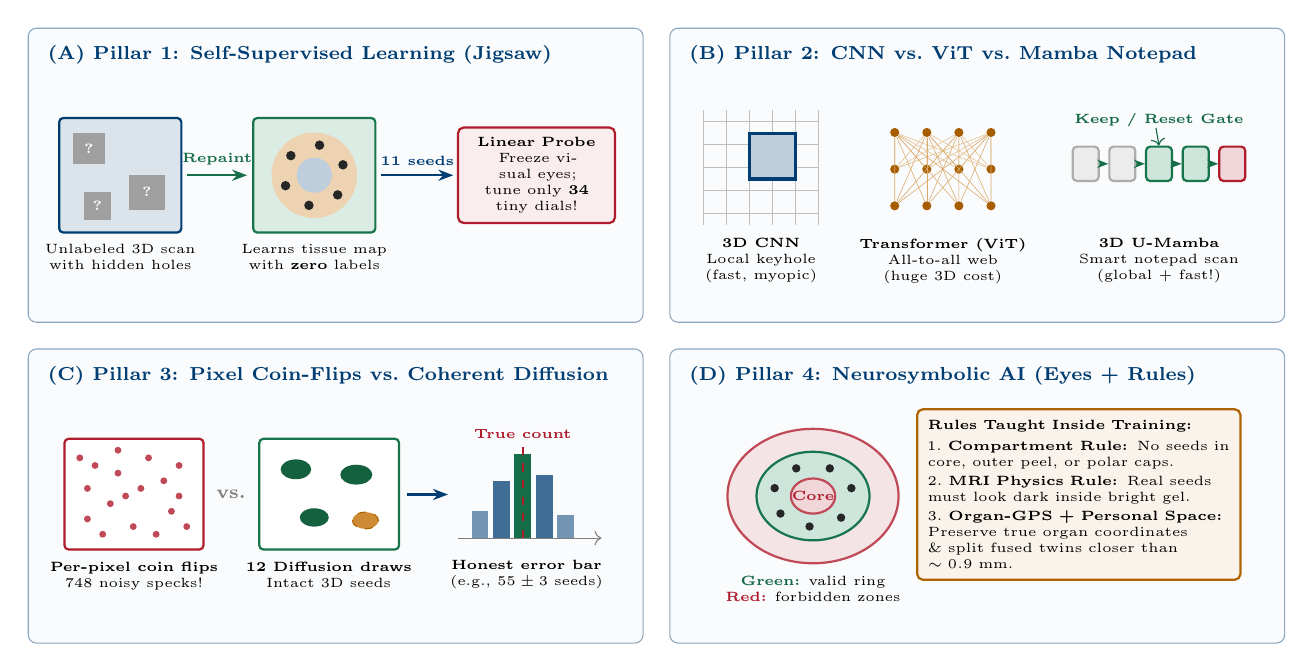
\begin{tikzpicture}[
    scale=0.97, transform shape,
    font=\scriptsize,
    panel/.style={rectangle, rounded corners=3pt, draw=uibblue!45, fill=lightgray!55, inner sep=4pt, minimum width=8.05cm, minimum height=3.85cm}
]
% --- PANEL A: 3D SSL Jigsaw ---
\node[panel] (pA) at (0,0) {};
\node[anchor=north west, font=\scriptsize\bfseries\color{uibblue}] at ([xshift=4pt,yshift=-3pt]pA.north west) {(A) Pillar 1: Self-Supervised Learning (Jigsaw)};

\begin{scope}[shift={(-3.62,-1.10)}]
    % Masked cube representation
    \fill[uibblue!14, draw=uibblue, thick, rounded corners=1.5pt] (0,0.35) rectangle (1.60,1.85);
    \fill[gray!75] (0.18,1.25) rectangle (0.60,1.65);
    \fill[gray!75] (0.92,0.65) rectangle (1.38,1.10);
    \fill[gray!75] (0.32,0.52) rectangle (0.68,0.88);
    \node[font=\tiny\bfseries, color=white] at (0.39,1.45) {?};
    \node[font=\tiny\bfseries, color=white] at (1.15,0.88) {?};
    \node[font=\tiny\bfseries, color=white] at (0.50,0.70) {?};
    \node[below, align=center, font=\tiny] at (0.80,0.32) {Unlabeled 3D scan\\with hidden holes};

    \draw[-{Stealth[length=1.9mm]}, thick, color=kiwigreen!80!black] (1.68,1.10) -- (2.46,1.10) node[midway, above, font=\tiny\bfseries\color{kiwigreen!75!black}] {Repaint};

    % Reconstructed anatomy
    \fill[kiwigreen!16, draw=kiwigreen!85!black, thick, rounded corners=1.5pt] (2.54,0.35) rectangle (4.14,1.85);
    \fill[amberwarn!30] (3.34,1.10) circle (0.56);
    \fill[uibblue!25] (3.34,1.10) circle (0.23);
    \foreach \ang in {20,80,140,200,260,320}{
        \fill[black!85] ({3.34+0.40*cos(\ang)},{1.10+0.40*sin(\ang)}) circle (0.062);
    }
    \node[below, align=center, font=\tiny] at (3.34,0.32) {Learns tissue map\\with \textbf{zero} labels};

    \draw[-{Stealth[length=1.9mm]}, thick, color=uibblue] (4.22,1.10) -- (5.16,1.10) node[midway, above, font=\tiny\bfseries\color{uibblue}] {11 seeds};

    % Tiny probe
    \node[rectangle, rounded corners=2pt, draw=uibred, fill=uibred!8, thick, align=center, font=\tiny, text width=1.82cm, minimum height=1.25cm] at (6.25,1.10) {\textbf{Linear Probe}\\Freeze visual eyes;\\tune only \textbf{34}\\tiny dials!};
\end{scope}

% --- PANEL B: CNN vs ViT vs Mamba ---
\node[panel] (pB) at (8.40,0) {};
\node[anchor=north west, font=\scriptsize\bfseries\color{uibblue}] at ([xshift=4pt,yshift=-3pt]pB.north west) {(B) Pillar 2: CNN vs.\ ViT vs.\ Mamba Notepad};

\begin{scope}[shift={(4.82,-1.10)}]
    % CNN Keyhole
    \draw[gray!50, step=0.30] (0,0.45) grid (1.50,1.95);
    \fill[uibblue!25, draw=uibblue, very thick] (0.60,1.05) rectangle (1.20,1.65);
    \node[below, align=center, font=\tiny] at (0.75,0.40) {\textbf{3D CNN}\\Local keyhole\\(fast, myopic)};

    % ViT All-to-All Web
    \foreach \i in {0,1,2,3}{
        \foreach \j in {0,1,2}{
            \node[circle, fill=amberwarn!85!black, inner sep=1.2pt] (v\i\j) at ({2.50+\i*0.42},{0.70+\j*0.48}) {};
        }
    }
    \foreach \i in {0,1,2,3}{
        \foreach \k in {0,1,2,3}{
            \draw[amberwarn!60, very thin] (v\i0) -- (v\k2);
            \draw[amberwarn!45, very thin] (v\i1) -- (v\k2);
        }
    }
    \node[below, align=center, font=\tiny] at (3.13,0.40) {\textbf{Transformer (ViT)}\\All-to-all web\\(huge 3D cost)};

    % Mamba Selective Notepad
    \foreach \t/\dcol/\fcol in {0/gray!65/gray!15, 1/gray!65/gray!15, 2/kiwigreen!85!black/kiwigreen!22, 3/kiwigreen!85!black/kiwigreen!22, 4/uibred/uibred!18}{
        \node[rectangle, rounded corners=1.5pt, draw=\dcol, fill=\fcol, thick, minimum width=0.34cm, minimum height=0.45cm] (m\t) at ({5.00+\t*0.48},1.25) {};
    }
    \foreach \t [evaluate=\t as \tn using int(\t+1)] in {0,1,2,3}{
        \draw[-{Stealth[length=1.4mm]}, thick, color=kiwigreen!80!black] (m\t) -- (m\tn);
    }
    \node[font=\tiny\bfseries, color=kiwigreen!75!black] at (5.96,1.82) {Keep / Reset Gate};
    \draw[->, thin, color=kiwigreen!75!black] (5.92,1.72) -- (m2.north);
    \node[below, align=center, font=\tiny] at (5.96,0.40) {\textbf{3D U-Mamba}\\Smart notepad scan\\(global + fast!)};
\end{scope}

% --- PANEL C: Diffusion Uncertainty ---
\node[panel] (pC) at (0,-4.20) {};
\node[anchor=north west, font=\scriptsize\bfseries\color{uibblue}] at ([xshift=4pt,yshift=-3pt]pC.north west) {(C) Pillar 3: Pixel Coin-Flips vs.\ Coherent Diffusion};

\begin{scope}[shift={(-3.55,-5.30)}]
    % Salt & pepper failure
    \fill[white, draw=uibred, thick, rounded corners=1.5pt] (0,0.40) rectangle (1.82,1.85);
    \foreach \x/\y in {0.2/1.6,0.4/1.5,0.3/1.2,0.7/1.4,0.6/1.0,1.1/1.6,1.3/1.3,1.5/1.5,1.4/0.9,0.9/0.7,0.5/0.6,1.2/0.6,1.6/0.7,0.8/1.1,1.0/1.2,0.3/0.8,1.5/1.1,0.7/1.7}{
        \fill[uibred!80] (\x,\y) circle (0.045);
    }
    \node[below, align=center, font=\tiny] at (0.91,0.36) {\textbf{Per-pixel coin flips}\\748 noisy specks!};

    % VS
    \node[font=\scriptsize\bfseries, color=gray] at (2.18,1.12) {vs.};

    % Coherent sculptor draws
    \fill[white, draw=kiwigreen!85!black, thick, rounded corners=1.5pt] (2.55,0.40) rectangle (4.38,1.85);
    \fill[kiwigreen!70!black] (3.03,1.45) ellipse (0.20 and 0.13);
    \fill[kiwigreen!70!black] (3.82,1.38) ellipse (0.21 and 0.13);
    \fill[kiwigreen!70!black] (3.27,0.82) ellipse (0.19 and 0.12);
    \fill[amberwarn!80, draw=amberwarn!90!black, dashed] (3.94,0.78) ellipse (0.17 and 0.11);
    \node[below, align=center, font=\tiny] at (3.46,0.36) {\textbf{12 Diffusion draws}\\Intact 3D seeds};

    % Arrow to histogram
    \draw[-{Stealth[length=1.9mm]}, thick, color=uibblue] (4.48,1.12) -- (5.02,1.12);

    % Count bell curve / bars
    \begin{scope}[shift={(5.15,0.55)}]
        \draw[->, thin, gray] (0,0) -- (1.88,0);
        \fill[uibblue!55] (0.18,0) rectangle (0.40,0.35);
        \fill[uibblue!75] (0.46,0) rectangle (0.68,0.75);
        \fill[kiwigreen!80!black] (0.74,0) rectangle (0.96,1.10);
        \fill[uibblue!75] (1.02,0) rectangle (1.24,0.82);
        \fill[uibblue!55] (1.30,0) rectangle (1.52,0.30);
        \draw[uibred, thick, dashed] (0.85,0) -- (0.85,1.22);
        \node[above, font=\tiny\bfseries, color=uibred] at (0.85,1.18) {True count};
        \node[below, align=center, font=\tiny] at (0.90,-0.16) {\textbf{Honest error bar}\\(e.g., $55 \pm 3$ seeds)};
    \end{scope}
\end{scope}

% --- PANEL D: Neurosymbolic + Organ-GPS ---
\node[panel] (pD) at (8.40,-4.20) {};
\node[anchor=north west, font=\scriptsize\bfseries\color{uibblue}] at ([xshift=4pt,yshift=-3pt]pD.north west) {(D) Pillar 4: Neurosymbolic AI (Eyes + Rules)};

\begin{scope}[shift={(4.95,-5.30)}]
    % Stylized kiwi cross-section
    \fill[uibred!12, draw=uibred!80, thick] (1.30,1.10) ellipse (1.12 and 0.88);
    \fill[kiwigreen!22, draw=kiwigreen!85!black, thick] (1.30,1.10) ellipse (0.74 and 0.58);
    \fill[uibred!18, draw=uibred!80, thick] (1.30,1.10) ellipse (0.29 and 0.23);
    \foreach \ang in {15,65,115,165,215,265,315}{
        \fill[black!85] ({1.30+0.52*cos(\ang)},{1.10+0.40*sin(\ang)}) circle (0.055);
    }
    \node[font=\tiny\bfseries, color=uibred] at (1.30,1.10) {Core};
    \node[below, align=center, font=\tiny] at (1.30,0.18) {\textcolor{kiwigreen!75!black}{\textbf{Green:}} valid ring\\ \textcolor{uibred}{\textbf{Red:}} forbidden zones};

    % Rules card on right
    \node[rectangle, rounded corners=2pt, draw=amberwarn!90!black, fill=amberwarn!8, thick, align=left, font=\tiny, text width=3.95cm, inner sep=4pt] at (4.78,1.12) {
        \textbf{Rules Taught Inside Training:}\\[2pt]
        1.~\textbf{Compartment Rule:} No seeds in core, outer peel, or polar caps.\\[1pt]
        2.~\textbf{MRI Physics Rule:} Real seeds must look dark inside bright gel.\\[1pt]
        3.~\textbf{Organ-GPS + Personal Space:} Preserve true organ coordinates \& split fused twins closer than $\sim 0.9\text{ mm}$.
    };
\end{scope}
\end{tikzpicture}
\caption{Visual intuition for the four frontier AI paradigms built in Notebook~\texttt{06}: (A)~Self-Supervised Learning builds anatomical understanding from unlabeled scans; (B)~3D U-Mamba sweeps globally with a selective memory notepad; (C)~Conditional Diffusion generates coherent 3D realizations to quantify count uncertainty; (D)~Neurosymbolic AI bakes anatomical and physical rules directly into network weights.}
\label{fig:nontech-frontier-intuition}
\end{figure}

\newpage
\subsection{Plain-English Definitions of Every Concept, Model \& Method}

\begin{table}[H]
\centering
\scriptsize
\renewcommand{\arraystretch}{1.18}
\rowcolors{2}{white}{rowalt}
\begin{tabularx}{\textwidth}{L{3.55cm} Y}
\toprule
\rowcolor{uibblue!14}
\textbf{Concept / Model} & \textbf{Plain-English Meaning \& Intuitive Analogy} \\
\midrule
\textbf{Self-Supervised Learning (\texttt{SSL}), \texttt{Models Genesis} \& \texttt{MAE}} & Teaching a network from \textbf{unlabeled} scans by creating an automatic ``fill-in-the-blank'' game (\emph{pretext task}): hide random 3D blocks of an MRI, add mild brightness jitter and noise, and ask the network to paint back the clean anatomy. To succeed, it must learn what organs, membranes, and seeds look like on its own. \\
\textbf{Inductive vs.\ Transductive \texttt{SSL}} & \textbf{Inductive} means strictly hiding the test region even during unlabeled pretraining (no peeking at the exam!); \textbf{transductive} lets the model see the unlabeled test scan first. We enforce inductive testing to prove genuine generalization. \\
\textbf{Emergent Features (\texttt{PCA $\to$ RGB}) \& Linear Probing} & After \texttt{SSL} pretraining, we can color every voxel by its top three learned internal patterns (\texttt{PCA $\to$ RGB}) and see distinct tissues emerge with zero labels. \textbf{Linear probing} freezes the entire pretrained brain and trains only a tiny handful of final decision weights (just 34 numbers!) on 11 labeled seeds. \\
\textbf{Selective State-Space Model (\texttt{Mamba}, \texttt{3D U-Mamba}, \texttt{SegMamba})} & Think of reading a long medical chart with a compact \textbf{smart notepad} (\emph{hidden state}). As \texttt{Mamba} sweeps across a 3D scan along three orthogonal directions (\emph{Tri-Oriented Scanning}), a learned \textbf{selective gate} decides at every voxel: \emph{``Is this a sharp new seed edge? Write it down and flush stale background!''} or \emph{``Still inside uniform gel? Hold onto long-range organ context!''} This gives global 3D vision without the huge memory cost of Transformers. \\
\textbf{Parallel Prefix Scan (No CUDA Lock-In)} & Reading voxels strictly one-by-one in Python is painfully slow, and official \texttt{Mamba} packages require proprietary NVIDIA-only code. A \textbf{parallel prefix scan} combines neighboring pairs simultaneously in a tournament-bracket tree (e.g., 13 fast parallel rounds instead of 6,400 slow sequential steps), giving the exact same result $30\times$ faster on MacBooks, Linux GPUs, and Colab alike. \\
\textbf{Conditional Diffusion \& Flow Matching (\texttt{MedSegDiff}, \texttt{CIMD})} & Instead of predicting one rigid mask, a generative diffusion/flow model starts from random static (fog) and smoothly \textbf{sculpts a complete, coherent 3D segmentation} over several quick refinement steps, guided by the MRI scan. Running this sculptor 12 times from different random starting fog produces 12 plausible 3D interpretations --- just like asking 12 independent radiologists! \\
\textbf{Aleatoric Uncertainty, Credible Intervals \& \texttt{AnoDDPM}} & \textbf{Aleatoric uncertainty} is genuine physical fuzziness in the image (e.g., thin seed poles blurred across thick MRI slices). Counting seeds across the 12 diffusion realizations gives a realistic \textbf{credible interval} (e.g., $55 \pm 3$ seeds) rather than shattered pixel noise. A related trick, \textbf{\texttt{AnoDDPM}}, trains only on healthy tissue and ``heals'' a diseased scan so anomalies pop out by subtraction. \\
\textbf{Out-of-Distribution (\texttt{OOD}) Collapse} & When an AI encounters anatomy it never saw during training (such as the polar tips or outer rind of the kiwifruit, or a new hospital scanner) and confidently hallucinates false lesions. \\
\textbf{Differentiable Neurosymbolic AI (\texttt{Logic Tensor Networks, LTN})} & Classic deep learning relies purely on pattern matching (\emph{neural}); textbooks rely on explicit rules (\emph{symbolic}). \textbf{\texttt{LTN}} translates textbook rules (``outside the inner ring $\Rightarrow$ not a seed''; ``seeds must be dark'') into smooth, trainable penalties applied on unlabeled regions. Using a strict ``for-all'' penalty ensures even a small pocket of wrong predictions is heavily corrected during training. \\
\textbf{\texttt{Organ-GPS} \& Hard-Core Clump Splitting} & Standard 3D CNN normalization (\texttt{InstanceNorm}) accidentally erases absolute position inside an organ by re-centering every local crop. Adding an un-normalized \textbf{\texttt{Organ-GPS}} side-branch tells the network where each voxel lies from center-to-rim and pole-to-equator. Finally, \textbf{hard-core splitting} uses Lab~5's physical finding that real seeds keep a minimum ``personal space'' ($\sim 0.9\text{ mm}$) to cleanly separate touching twin seeds. \\
\textbf{Beyond Voxel Grids: \texttt{INRs}, \texttt{GNNs} \& Object Queries} & Three bonus paradigms broaden your toolkit: \textbf{Implicit Neural Representations (\texttt{INRs}/\texttt{SIREN})} store a 3D scan as a smooth continuous formula (like vector graphics, free of blocky pixels); \textbf{Graph Neural Networks (\texttt{GNNs})} connect candidate seeds into a spatial constellation to spot radial patterns vs.\ stray vessels; \textbf{Object-Query Decoders (\texttt{DETR}/\texttt{Mask2Former})} dispatch learned ``detectives'' that each claim one instance directly without watershed heuristics. \\
\bottomrule
\end{tabularx}
\caption{Plain-English glossary of all frontier AI concepts, models, and methods introduced in this guide.}
\label{tab:nontech-frontier-defs}
\end{table}

\newpage
\subsection{Recommended Starting Resources (Reviews, Visual Guides, Repos, Videos \& Podcasts)}

Explore any of these accessible, well-illustrated starting points before diving into the mathematical formulations in Section~\ref{sec:frontier-pillars}:

\begin{table}[H]
\centering
\scriptsize
\renewcommand{\arraystretch}{1.22}
\rowcolors{2}{white}{rowalt}
\begin{tabularx}{\textwidth}{L{2.55cm} Y}
\toprule
\rowcolor{uibblue!14}
\textbf{Format} & \textbf{Curated Learning Resource (Clickable)} \\
\midrule
\textbf{Non-Technical Review Papers} &
$\bullet$ \href{https://doi.org/10.1038/s41746-023-00811-0}{\textbf{Huang et al., \emph{npj Digital Medicine} (2023)}} --- \emph{Self-supervised learning for medical image classification: systematic review \& guidelines}. \newline
$\bullet$ \href{https://doi.org/10.1016/j.media.2023.102846}{\textbf{Kazerouni et al., \emph{Medical Image Analysis} (2023)}} --- \emph{Diffusion models in medical imaging: A comprehensive survey}. \newline
$\bullet$ \href{https://link.springer.com/article/10.1007/s10462-023-10448-w}{\textbf{Garcez \& Lamb, \emph{Artificial Intelligence Review} (2023)}} (\href{https://arxiv.org/abs/2012.05876}{arXiv}) --- \emph{Neurosymbolic AI: The 3rd Wave} (accessible roadmap of neural + symbolic reasoning). \\
\textbf{Illustrated Tutorials \& Interactive Guides} &
$\bullet$ \href{https://newsletter.maartengrootendorst.com/p/a-visual-guide-to-mamba-and-state}{\textbf{Maarten Grootendorst: \emph{A Visual Guide to Mamba and State Space Models}}} --- 50+ crystal-clear diagrams explaining \texttt{Mamba} with zero pain! \newline
$\bullet$ \href{https://jalammar.github.io/illustrated-stable-diffusion/}{\textbf{Jay Alammar: \emph{The Illustrated Stable Diffusion}}} --- intuitive visual walkthrough of how diffusion sculpts images from noise. \newline
$\bullet$ \href{https://lilianweng.github.io/posts/2021-07-11-diffusion-models/}{\textbf{Lilian Weng (Lil'Log): \emph{What are Diffusion Models?}}} --- bridges intuition gently into the underlying equations. \newline
$\bullet$ \href{https://distill.pub/2021/gnn-intro/}{\textbf{Distill.pub: \emph{A Gentle Introduction to Graph Neural Networks}}} --- interactive visual explainer for spatial graphs (\texttt{GNNs}). \\
\textbf{Open-Source GitHub Repos} &
\href{https://github.com/bowang-lab/U-Mamba}{\texttt{bowang-lab/U-Mamba}} $\;\cdot\;$
\href{https://github.com/logictensornetworks/LTNtorch}{\texttt{logictensornetworks/LTNtorch}} $\;\cdot\;$
\href{https://github.com/logictensornetworks/logictensornetworks}{\texttt{logictensornetworks/logictensornetworks}} \\
\textbf{Videos \& Podcasts} &
$\bullet$ \href{https://www.youtube.com/watch?v=iv-5mZ_9CPY}{\textbf{3Blue1Brown (feat.\ Welch Labs): \emph{But how do AI images and videos actually work?}}} --- outstanding animated intuition for diffusion \& flow vector fields. \newline
$\bullet$ \href{https://www.youtube.com/playlist?list=PLZHQObOWTQDNU6R1_67000Dx_ZCJB-3pi}{\textbf{3Blue1Brown: \emph{Neural Networks / Deep Learning Playlist}}} --- foundational visual intuition if you want a quick refresher. \newline
$\bullet$ \href{https://ai-podcast.nejm.org/}{\textbf{NEJM AI Grand Rounds}} \& \href{https://twimlai.com/}{\textbf{The TWIML AI Podcast}} --- accessible interviews on medical AI, uncertainty, self-supervision, and state-space models. \\
\bottomrule
\end{tabularx}
\caption{Curated non-technical reviews, visual tutorials, GitHub repositories, videos, and podcasts for the frontier paradigms in Notebook~\texttt{06}.}
\label{tab:nontech-frontier-resources}
\end{table}

% =====================================================================
% SECTION 2: COMPLETING THE 6-PILLAR TAXONOMY
% =====================================================================
\section{Completing the 6-Pillar Biomedical AI Landscape (Notebooks 04--06)}

In \textbf{Notebook \texttt{04}} (3D Semantic \& Multi-Task Instance U-Nets) and \textbf{Notebook \texttt{05}} (\texttt{SAM 2.1} \& \texttt{MedSAM} Vision Foundation Models), we studied the two most widely deployed deep architectures in medical image analysis: \textbf{3D Convolutional Neural Networks (\texttt{CNNs})} and \textbf{Promptable Vision Transformers (\texttt{ViTs})}. Yet four fundamental bottlenecks still arise across real clinical imaging and 3D microscopy studies:

\begin{enumerate}
    \item \textbf{Extreme Label Scarcity ($99.4\%$ Unlabeled Organ Voxels) $\rightarrow$ 3D Self-Supervised Learning (\texttt{SSL}):} Our 7T kiwifruit scan contains $8{,}388{,}608$ voxels, whereas expert 3D instance labels cover $<0.6\%$. When a clinician annotates only a tiny $24 \times 20 \times 6$ micro-box ($11$ seeds), training a $340\text{k}$-parameter 3D CNN from scratch overfits severely (\texttt{PQ = 0.209}).
    \item \textbf{Local CNN Blindness vs.\ Quadratic $\mathcal{O}(N^2)$ ViT Cost $\rightarrow$ Selective State-Space Models (\texttt{3D U-Mamba}):} Local $3\times 3\times 3$ convolutions have a small receptive field, while global 3D self-attention scales as $\mathcal{O}(N^2)$, forcing coarse $16\times 16$ patching (\texttt{Trap 1} in Notebook \texttt{05}). Selective State-Space Models scan global 3D volumes in $\mathcal{O}(N)$ memory and $\mathcal{O}(\log L)$ parallel depth.
    \item \textbf{Point Estimates Hide Ambiguity $\rightarrow$ Conditional Diffusion / Flow Matching:} Challenge Task~1 requires an \textbf{uncertainty range} on seed count $N$, and Notebook~\texttt{03b} showed human inter-rater disagreement on partial-volume polar tips ($\Delta z = 0.50\text{ mm}$) and kissing seed pairs. Sampling independent pixels from U-Net softmax probabilities shatters into $748$ salt-and-pepper specks instead of plausible 3D seeds.
    \item \textbf{Spatial Out-of-Distribution (\texttt{OOD}) Collapse $\rightarrow$ Differentiable Neurosymbolic AI (\texttt{LTN}):} Sliding an equatorial-trained 3D CNN across all 128 whole-fruit slices triggers \textbf{$5{,}571$ unmasked blobs ($132{,}275$ OOD false-positive voxels!)} on oblique polar vascular bundles and outer-cortex parenchyma.
\end{enumerate}

\newpage
\subsection{Architectural Rosetta Stone: Comparing the 6 Runnable AI Pillars}

\begin{table}[H]
\centering
\scriptsize
\renewcommand{\arraystretch}{1.22}
\rowcolors{2}{white}{rowalt}
\begin{tabularx}{\textwidth}{L{2.25cm} Y Y Y Y Y}
\toprule
\rowcolor{uibblue!14}
\textbf{Pillar} & \textbf{Core Primitive} & \textbf{Spatial Scope \& Cost} & \textbf{Supervision Needed} & \textbf{Uncertainty / OOD} & \textbf{Kiwi Highlight} \\
\midrule
\textbf{1. 3D ConvNet} (\emph{NB 04 U-Net}) & $3\times 3\times 3$ local convolutions & Local ($\mathcal{O}(N)$) & Moderate ($59$ seeds) & Marginal $p(\mathbf{x})$; $132\text{k}$ OOD vox & Fast sharp edges (\texttt{SQ = 0.698}, \texttt{PQ = 0.395}) \\
\textbf{2. Promptable ViT} (\emph{NB 05 SAM 2.1}) & $16\times 16$ tokens + cross-attn + memory & Global 2D ($\mathcal{O}(N^2)$) & \textbf{Zero labels} (prompts) & Scalar $\widehat{\text{IoU}}$; needs external ring gate & 1-Click 3D curation (\texttt{PQ = 0.500}) \\
\textbf{3. 3D SSL} (\emph{Models Genesis / MAE}) & 35\% cuboid mask \& contrast restoration & Meso-scale ($\mathcal{O}(N)$) & \textbf{11 seeds + 34 probe params!} & Emergent zero-label tissue PCA & \textbf{$+40.7\%$ scarce-label \texttt{PQ} ($\mathbf{0.209 \rightarrow 0.294}$)} \\
\textbf{4. 3D State-Space} (\emph{U-Mamba / S6}) & Input-selective scan $\mathbf{h}_t = \bar{\mathbf{A}}_t\mathbf{h}_{t-1} + \bar{\mathbf{B}}_t\mathbf{x}_t$ & \textbf{Global 3D ($\mathcal{O}(N)$ mem, $\mathcal{O}(\log L)$ time)} & Moderate ($59$ seeds) & Learned boundary gate $\Delta_t(\mathbf{x})$ & \textbf{Exact 52/52 count, 0 splits, \texttt{SQ = 0.696}} \\
\textbf{5. Cond.\ Diffusion} (\emph{MedSegDiff / CIMD}) & Velocity ODE $\frac{d\mathbf{Y}_t}{dt} = \mathbf{v}_\theta(\mathbf{Y}_t, t \mid \mathcal{F}_\phi(\mathbf{X}))$ & Joint 3D field ($S \times \mathcal{O}(N)$) & Moderate ($59$ seeds) & \textbf{Posterior $P(N\mid\mathbf{X}) = 54.6 \pm 3.1$} & \textbf{Brackets \texttt{GT=52}; ensemble \texttt{PQ = 0.447}} \\
\textbf{6. Neurosymbolic} (\emph{LTN + Organ-GPS}) & Neural backbone + $p$-mean logic + split & Local + \textbf{Global GPS $(r/R, z/Z)$} & $59$ seeds + $40$ unlab cubes & \textbf{0 polar cap FP voxels ($-100\%$!)} & \textbf{Best automated \texttt{PQ = 0.508}, \texttt{SQ = 0.763}} \\
\bottomrule
\end{tabularx}
\caption{Division of labor across the 6 runnable biomedical segmentation pillars in Notebooks \texttt{04}--\texttt{06}.}
\end{table}

\begin{figure}[H]
\centering
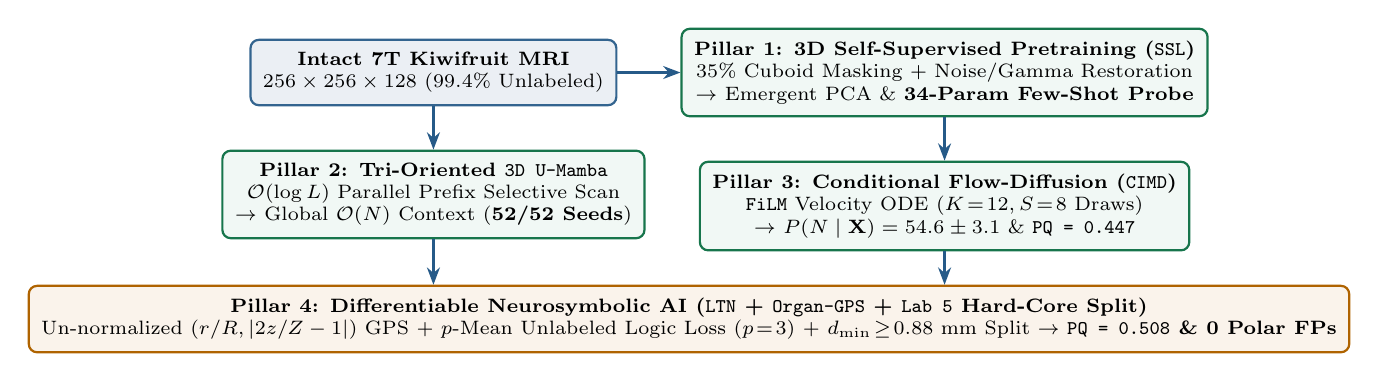
\begin{tikzpicture}[
    node distance=0.45cm and 0.65cm,
    box/.style={rectangle, rounded corners=3pt, draw=uibblue!80, fill=white, thick, align=center, font=\scriptsize, inner sep=4.5pt},
    pbox/.style={rectangle, rounded corners=3pt, draw=kiwigreen!85!black, fill=kiwigreen!6, thick, align=center, font=\scriptsize, inner sep=4.5pt},
    arr/.style={-{Stealth[length=2.2mm]}, thick, color=uibblue!85}
]
    \node[box, fill=uibblue!8, minimum width=4.4cm] (raw) {\textbf{Intact 7T Kiwifruit MRI}\\$256\times 256\times 128$ ($99.4\%$ Unlabeled)};
    \node[pbox, right=0.8cm of raw, minimum width=5.2cm] (ssl) {\textbf{Pillar 1: 3D Self-Supervised Pretraining (\texttt{SSL})}\\35\% Cuboid Masking + Noise/Gamma Restoration\\$\rightarrow$ Emergent PCA \& \textbf{34-Param Few-Shot Probe}};
    \node[pbox, below=0.55cm of raw, minimum width=4.4cm] (ssm) {\textbf{Pillar 2: Tri-Oriented \texttt{3D U-Mamba}}\\\textbf{$\mathcal{O}(\log L)$} Parallel Prefix Selective Scan\\$\rightarrow$ Global $\mathcal{O}(N)$ Context (\textbf{52/52 Seeds})};
    \node[pbox, below=0.55cm of ssl, minimum width=5.2cm] (diff) {\textbf{Pillar 3: Conditional Flow-Diffusion (\texttt{CIMD})}\\\texttt{FiLM} Velocity ODE ($K\!=\!12, S\!=\!8$ Draws)\\$\rightarrow$ \textbf{$P(N\mid\mathbf{X}) = 54.6 \pm 3.1$} \& \textbf{\texttt{PQ = 0.447}}};
    \node[box, fill=amberwarn!8, draw=amberwarn!90!black, below=0.50cm of $(ssm.south)!0.5!(diff.south)$, minimum width=10.4cm] (ltn) {\textbf{Pillar 4: Differentiable Neurosymbolic AI (\texttt{LTN} + \texttt{Organ-GPS} + \texttt{Lab 5} Hard-Core Split)}\\Un-normalized $(r/R, \lvert 2z/Z - 1\rvert)$ GPS + $p$-Mean Unlabeled Logic Loss ($p\!=\!3$) + $d_{\min}\!\ge\!0.88\text{ mm}$ Split $\rightarrow$ \textbf{\texttt{PQ = 0.508} \& 0 Polar FPs}};

    \draw[arr] (raw) -- (ssl);
    \draw[arr] (raw) -- (ssm);
    \draw[arr] (ssl) -- (diff);
    \draw[arr] (ssm.south) -- (ssm.south |- ltn.north);
    \draw[arr] (diff.south) -- (diff.south |- ltn.north);
\end{tikzpicture}
\caption{How the four pure-PyTorch frontier paradigms in Notebook \texttt{06} build upon the 2005 UiB 7T MRI scan.}
\end{figure}

% =====================================================================
% SECTION 2: MATHEMATICAL DEEP DIVES INTO PILLARS 1--4
% =====================================================================
\section{Mathematical \& Biophysical Foundations of the Four Frontier Pillars}
\label{sec:frontier-pillars}

\subsection{Pillar 1 --- 3D Self-Supervised Learning (\texttt{Models Genesis} \& \texttt{3D MAE})}

Given $36$ unlabeled $64\times 40\times 16$ cubes $\mathcal{D}_U$ sampled across the whole kiwifruit (\textbf{strictly disjoint} from the held-out test wedge $[128\!:\!208,\, 168\!:\!208,\, 56\!:\!72]$ to guarantee inductive evaluation), we apply a stochastic corruption operator $\tilde{\mathbf{X}} = \mathcal{C}(\mathbf{X}; \mathbf{M}, \gamma, \boldsymbol{\eta})$ combining $35\%$ 3D cuboid block masking ($\mathbf{M}$ at $4\times 4\times 2$ seed scale), gamma contrast jitter ($I^\gamma, \gamma \in [0.80, 1.25]$), and Rician-scale noise. A lightweight pretext head $g_\psi$ atop \texttt{Backbone3DUNet} $f_\theta$ reconstructs clean $T_2$ intensity, local mucilage-to-seed contrast drop, and 3D LoG blobness:
\begin{equation}
    \mathcal{L}_{\text{SSL}}(\theta, \psi) = \mathbb{E}_{\mathbf{X}\sim\mathcal{D}_U}\!\left[\big\lVert (1 + 2\mathbf{M})(1 + 3\mathbf{Y}_{\text{LoG}}) \odot \big(g_\psi(f_\theta(\tilde{\mathbf{X}})) - \mathbf{Y}_{\text{self}}\big) \big\rVert_2^2\right].
\end{equation}
Projecting the frozen 16-channel embeddings onto 3 principal components (\texttt{PCA $\rightarrow$ RGB}, Fig.~\ref{fig:frontier-bench}B) reveals \textbf{zero-label tissue parcellation} separating \emph{columella}, \emph{locular mucilage}, \emph{outer cortex}, and \emph{seeds}. On a tiny $11$-seed micro-box ($0.034\%$ of the scan), freezing all $340{,}416$ encoder weights and fitting \textbf{only $34$ linear-probe parameters} eliminates all split errors ($7 \rightarrow 0$) and raises \texttt{PQ} by \textbf{$+40.7\%$ (\texttt{0.209} $\rightarrow$ \texttt{0.294})}!

\subsection{Pillar 2 --- Selective State-Space Models (\texttt{3D U-Mamba} via \texorpdfstring{$\mathcal{O}(\log_2 L)$}{O(log2 L)} Associative Scan)}

In \textbf{Mamba (\texttt{S6})} \cite{gu2024mamba} and \textbf{\texttt{U-Mamba} / \texttt{SegMamba}} \cite{ma2024umamba,xing2024segmamba}, a 1D sequence of 3D feature tokens $\mathbf{x}_1, \dots, \mathbf{x}_L \in \mathbb{R}^C$ updates a latent state $\mathbf{h}_t \in \mathbb{R}^{C\times N}$ via input-dependent zero-order hold discretization:
\begin{equation}
    \Delta_t = \operatorname{softplus}(\mathbf{W}_\Delta \mathbf{x}_t + b_\Delta), \qquad \bar{\mathbf{A}}_t = \exp(\Delta_t \mathbf{A}), \qquad \mathbf{h}_t = \bar{\mathbf{A}}_t \odot \mathbf{h}_{t-1} + (\Delta_t \mathbf{x}_t) \otimes \mathbf{B}_t.
\end{equation}
\begin{warningbox}[Hardware Portability: Solving the \texttt{mamba-ssm} CUDA C++ Lock-In]
Official \texttt{mamba-ssm} wheels require proprietary NVIDIA CUDA C++ kernels and fail on macOS Apple Silicon (\texttt{MPS}) and CPU, whereas a naive Python \texttt{for t in range(L):} loop over $L = 6{,}400$ tokens takes $>300\text{ s}$! Because affine linear maps $f_t(h) = a_t h + b_t$ compose \textbf{associatively} --- $(a_2, b_2) \circ (a_1, b_1) = (a_2 a_1,\, a_2 b_1 + b_2)$ --- our pure-PyTorch \textbf{Hillis--Steele parallel prefix scan} computes all $L$ states in $\lceil \log_2 L \rceil \le 13$ vectorized GPU ops (\textbf{$30\times$ speedup: $302\text{ s} \rightarrow 9.89\text{ s}$ on M4 Max \texttt{mps}}), recovering \textbf{52/52 test seeds with 0 split errors (\texttt{SQ = 0.696})}.
\end{warningbox}

\subsection{Pillar 3 --- Conditional Flow-Matching Diffusion (\texttt{MedSegDiff} / \texttt{CIMD})}

Drawing independent Bernoulli pixels from a U-Net softmax map produces \textbf{$748$ noisy 1-voxel specks} on the $80\times 40\times 16$ test wedge because marginal probabilities ignore spatial covariance. Instead, we formulate generative segmentation via \textbf{Continuous-Time Conditional Flow Matching (\texttt{CFM})} \cite{wu2024medsegdiff,rahman2023cimd,liu2023flow} over joint 2-channel fields $\mathbf{Y}_1 = 2[\mathbf{M}_{\text{sem}}, \mathbf{D}_{\text{norm}}] - 1 \in [-1, +1]^{2\times X\times Y\times Z}$, interpolating $\mathbf{Y}_t = (1-t)\boldsymbol{\epsilon} + t\mathbf{Y}_1$ ($\boldsymbol{\epsilon}\sim\mathcal{N}(\mathbf{0}, \sigma^2\mathbf{I})$) and training a \texttt{FiLM}-modulated 3D velocity network:
\begin{equation}
    \mathcal{L}_{\text{CFM}}(\theta, \phi) = \mathbb{E}_{t\sim\mathcal{U}(0,1),\,\boldsymbol{\epsilon}}\!\left[\big\lVert w_{\text{fg}} \odot \big(\mathbf{v}_\theta(\mathbf{Y}_t, t \mid \mathcal{F}_\phi(\mathbf{X})) - (\mathbf{Y}_1 - \boldsymbol{\epsilon})\big) \big\rVert_2^2\right].
\end{equation}
Caching $\mathcal{F}_\phi(\mathbf{X}_{\text{test}})$ once allows sampling $K=12$ coherent 3D realizations ($S=8$ Euler steps) in \textbf{$0.22\text{ s}$}:
\begin{itemize}
    \item \textbf{Calibrated Count Credible Interval:} $P(N\mid\mathbf{X})$ yields \textbf{$54.6 \pm 3.1$ seeds ($90\%$ CI $[51, 60]$)}, cleanly bracketing \textbf{$\text{GT} = 52$} (Fig.~\ref{fig:frontier-bench}C)!
    \item \textbf{Aleatoric Uncertainty \& Accuracy:} $\sigma_{\text{diff}}(\mathbf{x})$ highlights partial-volume seed poles and kissing clefts (mirroring human \texttt{STAPLE} disagreement in Notebook~\texttt{03b}), while the posterior ensemble achieves \textbf{\texttt{PQ = 0.447} (\texttt{Dice = 0.682}, \texttt{RQ = 0.673})}.
\end{itemize}

\subsection{Pillar 4 --- Differentiable Neurosymbolic AI (\texttt{LTN} + \texttt{Organ-GPS} + Hard-Core Split)}

In \textbf{Logic Tensor Networks (\texttt{LTN})} \cite{badreddine2022ltn}, botanical and MRI-physics rules become smooth real-logic penalties over $40$ stratified unlabeled whole-fruit cubes $\Omega_U$ (covering polar caps, outer cortex, central \emph{columella}, and equator):
\begin{equation}
    \mathcal{L}_{\text{logic}}(\theta) = \lambda_1 \mathcal{L}_{\forall, p}\!\Big(\big(1 - R_{\text{ring}}(\mathbf{x})\big)\,p_\theta(\mathbf{x})\Big) + \lambda_2 \mathcal{L}_{\forall, p}\!\Big(p_\theta(\mathbf{x})\,B_{\text{non-dark}}(\mathbf{x})\Big), \qquad \mathcal{L}_{\forall, p}(v) = \left(\frac{1}{\lvert\Omega_U\rvert}\sum_{\mathbf{x}\in\Omega_U} v(\mathbf{x})^p + \varepsilon\right)^{\!1/p}\!\!.
\end{equation}
\begin{infobox}[Crucial Architectural Lesson: Why \texttt{InstanceNorm3d} Erases Organ Coordinates]
Passing organ coordinates $(r/R, \lvert 2z/Z - 1\rvert)$ into standard \texttt{nnU-Net} \texttt{InstanceNorm3d} layers standardizes every local patch to zero mean and unit variance --- mapping polar patches ($z \in [0, 16]$) and equatorial patches ($z \in [56, 72]$) onto the \emph{exact same} $[-1.7, +1.7]$ range! Routing $[r/R,\, (r/R - 0.43)^2,\, \lvert 2z/Z - 1\rvert]$ through an \textbf{un-normalized $1\times 1\times 1$ \texttt{Organ-GPS} MLP} preserves metric coordinates, while declarative \textbf{Lab~5 Mat\'ern hard-core clump splitting} ($d_{\min} \ge 0.88\text{ mm}$) resolves fused twins.
\end{infobox}

% =====================================================================
% SECTION 3: ADDITIONAL SOTA FAMILIES BEYOND VOXEL GRIDS
% =====================================================================
\section{Beyond Voxel Grids: Three Complementary SOTA Families}

In addition to our six voxel- and slice-based pillars, three non-grid/set-based families bridge directly to Labs~1, 3, and~5:

\begin{table}[H]
\centering
\scriptsize
\renewcommand{\arraystretch}{1.22}
\rowcolors{2}{white}{rowalt}
\begin{tabularx}{\textwidth}{L{3.2cm} Y Y L{2.8cm}}
\toprule
\rowcolor{uibblue!14}
\textbf{Frontier Family} & \textbf{Core Mathematical Mechanism} & \textbf{Role on Anisotropic 7T Kiwi Seeds} & \textbf{BMED365 Bridge} \\
\midrule
\textbf{Implicit Neural Fields (\texttt{INRs} / \texttt{SIREN})} \cite{sitzmann2020siren} & Continuous coordinate MLP $f_\theta(x_{\text{mm}}, y_{\text{mm}}, z_{\text{mm}})$ with periodic $\sin(\omega_0\mathbf{W}\mathbf{x})$ activations & Resolution-free continuous representation bridging $0.234\text{ mm}$ $(x,y)$ vs.\ $0.500\text{ mm}$ $z$ anisotropy without grid resampling artifacts & \textbf{Lab~5 \texttt{PINNs}} \& inverse problems (\emph{NB 02}) \\
\textbf{Spatial Graph Neural Nets (\texttt{GNNs} / \texttt{PyG})} & Candidate 3D centroids form graph $G=(V,E)$ ($r \le 2.5\text{ mm}$); relational message passing over locular geometry & Distinguishes true seeds arranged along $\sim 33$ radial locules ($d_{\min}\approx 0.95\text{ mm}$) from collinear vascular bundle false positives & \textbf{Lab~1 Network Science} (\texttt{torch-geometric} pre-installed!) \\
\textbf{Object-Query Set Decoders (\texttt{Mask2Former}) \& VLMs} & $Q$ learnable query tokens cross-attend to 3D features with Hungarian bipartite matching; Agentic LLM tool loops & Eliminates heuristic watershed post-processing on local patches; multimodal LLMs orchestrate Python verification dashboards & \textbf{Lab~3 GenAI / Agents} \& \textbf{NB 05 Mask Tokens} \\
\bottomrule
\end{tabularx}
\caption{Complementary non-grid and set-based SOTA paradigms across the BMED365 curriculum.}
\end{table}

% =====================================================================
% SECTION 4: EMPIRICAL BENCHMARK & REPRODUCIBLE RECIPES
% =====================================================================
\newpage
\section{Empirical Benchmark on the 2005 UiB 7T Kiwi MRI}

All experiments below run end-to-end in $\sim 70\text{ s}$ on an Apple MacBook Pro M4 Max (\texttt{mps}) or Google Colab \texttt{T4} GPU in Notebook~\texttt{06}:

\begin{figure}[H]
    \centering
    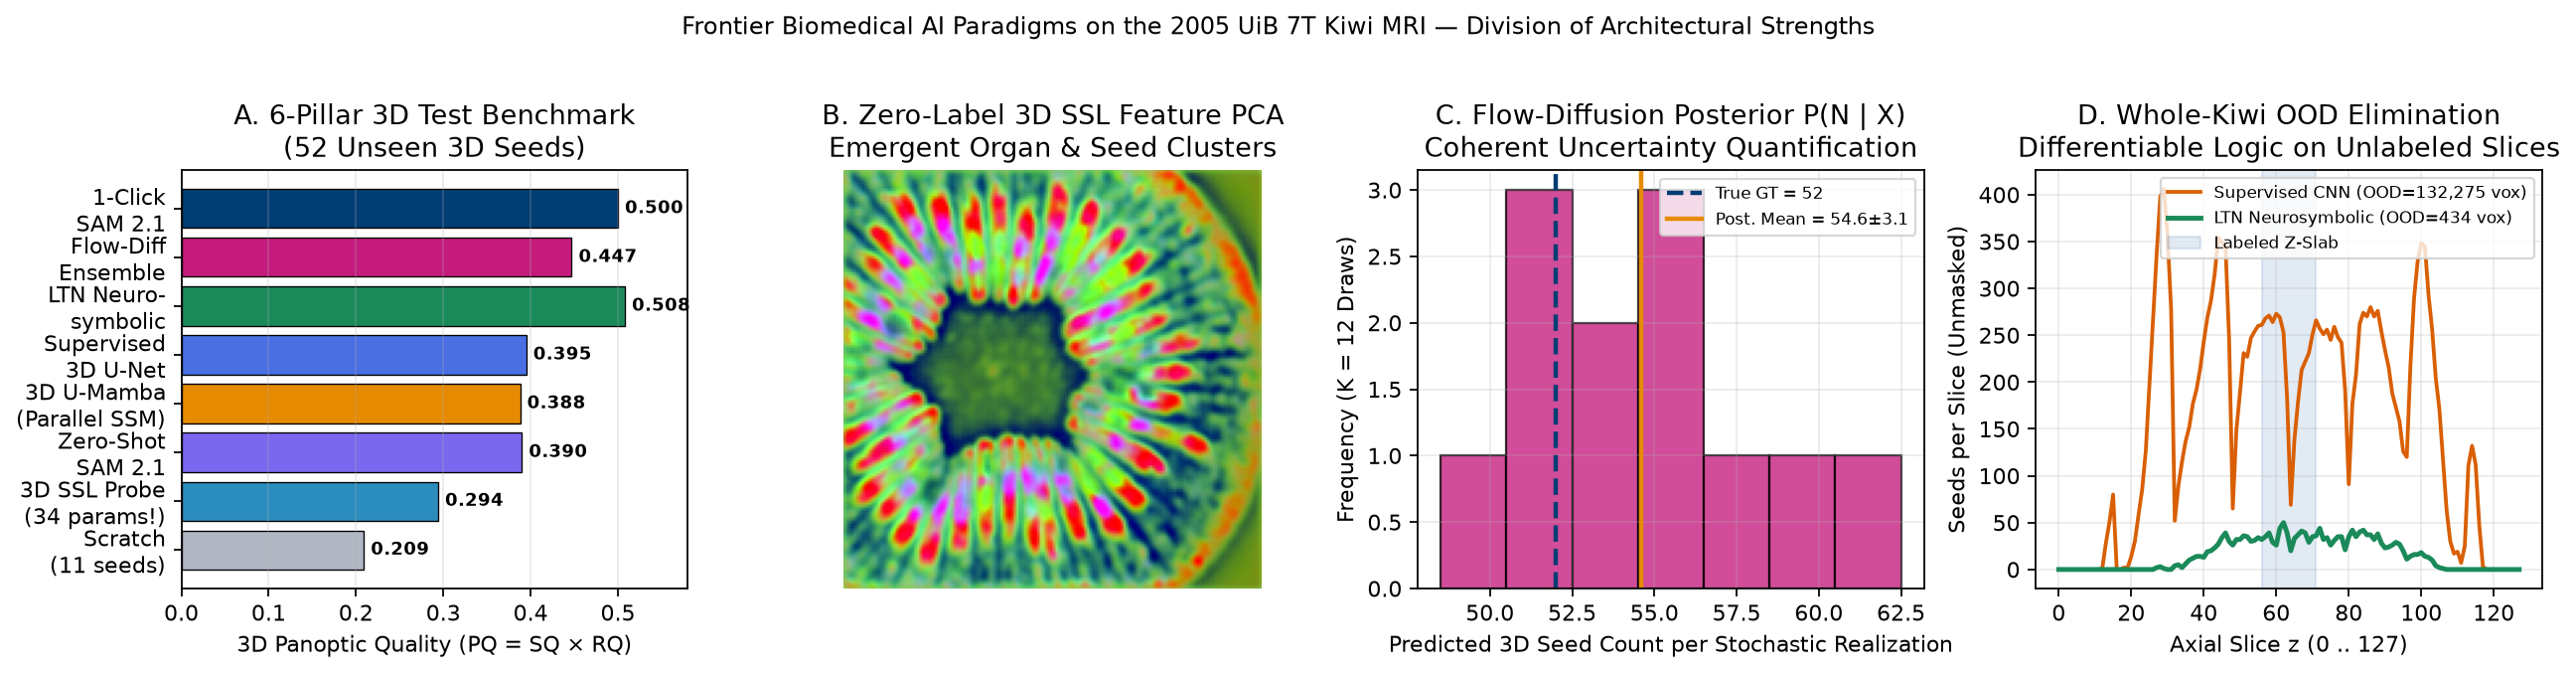
\includegraphics[width=\textwidth]{../assets/kiwi_frontier_paradigms_benchmark.png}
    \caption{Empirical benchmark executed in Notebook~\texttt{06} on Apple MacBook Pro M4 Max (\texttt{mps}, \texttt{float32}): (A)~6-pillar Panoptic Quality progression on the 52-seed held-out test wedge; (B)~zero-label 3D SSL feature PCA parcellation; (C)~calibrated Flow-Diffusion seed-count posterior $P(N\mid\mathbf{X})$ bracketing $\text{GT}=52$; (D)~complete elimination of polar OOD false positives by LTN differentiable logic without post-hoc masks.}
    \label{fig:frontier-bench}
\end{figure}

\begin{table}[H]
\centering
\scriptsize
\renewcommand{\arraystretch}{1.18}
\rowcolors{2}{white}{rowalt}
\begin{tabularx}{\textwidth}{Y C{1.55cm} C{1.05cm} C{0.82cm} C{0.82cm} C{0.72cm} C{0.78cm} C{0.85cm} C{0.80cm} R{1.45cm}}
\toprule
\rowcolor{uibblue!14}
\textbf{AI Paradigm \& Training Regime} & \textbf{Supervision} & \textbf{Pred ($\text{GT}\!=\!52$)} & \textbf{Sem.\ Dice} & \textbf{Merge} & \textbf{Split} & \textbf{SQ} & \textbf{RQ ($F_1$)} & \textbf{PQ} & \textbf{Time (\texttt{mps})} \\
\midrule
1. Scratch 3D Multi-Task U-Net ($11$-seed box) & 11 seeds ($340\text{k}$) & 113 & 0.402 & 4 & 7 & 0.540 & 0.388 & 0.209 & $4.5\text{ s}$ \\
\textbf{2. \texttt{3D SSL} Frozen Linear Probe ($11$-seed box)} & \textbf{11 seeds (34 params!)} & 78 & 0.419 & 6 & \textbf{0} & 0.579 & \textbf{0.508} & \textbf{0.294} & $11.4\text{ s}$ SSL \\
3. Zero-Shot Batched \texttt{SAM 2.1} + Gate (\emph{NB 05}) & \textbf{0 labels, 0 clicks} & 43 & 0.617 & 3 & \textbf{0} & 0.618 & 0.632 & 0.390 & $2.2\text{ s}$ \\
4. Supervised 3D Multi-Task U-Net (\emph{NB 04}) & 59 seeds (wedge) & 54 & 0.663 & 4 & 1 & 0.698 & 0.566 & 0.395 & $6.2\text{ s}$ \\
5. \texttt{3D SSL} Pretrained + Fine-Tuned U-Net & 59 seeds + SSL & \textbf{52} & 0.645 & 3 & \textbf{0} & 0.666 & 0.577 & 0.384 & $17.4\text{ s}$ \\
\textbf{6. Tri-Oriented \texttt{3D U-Mamba} ($\mathcal{O}(\log L)$ SSM)} & 59 seeds (wedge) & \textbf{52} & 0.653 & 4 & \textbf{0} & \textbf{0.696} & 0.558 & 0.388 & $9.9\text{ s}$ \\
\textbf{7. Conditional Flow-Diffusion ($K\!=\!12, S\!=\!8$)} & 59 seeds + $P(N\mid\mathbf{X})$ & 58 ($54.6\!\pm\!3.1$) & 0.682 & 5 & 1 & 0.665 & \textbf{0.673} & \textbf{0.447} & $24.1\text{ s} / 0.22\text{ s}$ \\
\textbf{8. \texttt{LTN} Neurosymbolic + Split (NO test mask!)} & 59 seeds + 40 unlab & 35 & \textbf{0.717} & \textbf{2} & \textbf{0} & \textbf{0.763} & 0.667 & \textbf{0.508} & $22.6\text{ s}$ \\
9. Interactive 1-Click/Seed \texttt{SAM 2.1} (\emph{NB 05}) & 52 human clicks & \textbf{52} & \textbf{0.761} & 4 & 4 & 0.565 & \textbf{0.885} & \textbf{0.500} & $23.0\text{ s}$ \\
\bottomrule
\end{tabularx}
\caption{Unified 3D instance benchmark on the held-out $80\times 40\times 16$ test wedge ($\text{GT}=52$ unseen 3D seeds, Hungarian matching at $\text{IoU}\ge 0.25$). Unmasked whole-kiwi ($256\times 256\times 128$) inference: Supervised U-Net produces $5{,}571$ blobs ($132{,}275$ OOD voxels, $9{,}581$ polar FP voxels) vs.\ \texttt{LTN} Neurosymbolic's \textbf{$0$ polar FP voxels} ($434$ OOD voxels, $-99.7\%$, Micro-GT calibrated $\widehat{N}_{\text{cal}} = 1{,}217$ seeds in $0.99\text{ s}$).}
\end{table}

\section{Minimal Pure-PyTorch Recipes \& Self-Check Q\&A}

\begin{lstlisting}[style=pybmed]
import math, torch, torch.nn as nn

def parallel_linear_scan(a: torch.Tensor, b: torch.Tensor) -> torch.Tensor:
    """Exact Hillis-Steele O(log2 L) parallel prefix scan for h_t = a_t * h_{t-1} + b_t (CUDA, MPS & CPU native)."""
    L = a.shape[1]
    for k in range(int(math.ceil(math.log2(max(L, 2))))):
        stride = 1 << k
        if stride >= L: break
        b = torch.cat([b[:, :stride], a[:, stride:] * b[:, :-stride] + b[:, stride:]], dim=1)
        a = torch.cat([a[:, :stride], a[:, stride:] * a[:, :-stride]], dim=1)
    return b

def ltn_universal_pmean(violation: torch.Tensor, p: float = 3.0) -> torch.Tensor:
    """Logic Tensor Network (LTN) ForAll quantifier: strongly penalizes localized OOD axiom counterexamples."""
    return (torch.mean(violation.clamp(0.0, 1.0) ** p) + 1e-8) ** (1.0 / p)
\end{lstlisting}

\begin{qabox}[Check Your Understanding: Generative Uncertainty vs.\ Softmax Sampling]
\textbf{Question:} Why does independent Bernoulli sampling from U-Net probabilities ($m_{\mathbf{x}} \sim \operatorname{Bernoulli}(p(\mathbf{x}))$) fail to estimate seed-count uncertainty ($748$ specks), whereas Conditional Flow-Diffusion succeeds ($54.6 \pm 3.1$, bracketing $\text{GT}=52$)?\\[2pt]
\textbf{Answer:} 3D object count is a non-local topological functional. Independent voxel draws ignore spatial covariance across boundary rims, shattering uncertain edges into single-voxel dust. Conditional Flow-Diffusion integrates shared noise fields through $3\times 3\times 3$ \texttt{FiLM} residual blocks, coherently toggling ambiguous seed poles or bridges as intact 3D instances.
\end{qabox}

\begin{thebibliography}{9}
\scriptsize
\setlength{\itemsep}{1.5pt}
    \bibitem{zhou2021} Zhou Z et al. \emph{Models Genesis.} \textbf{Medical Image Analysis} 67:101840 (2021). \href{https://doi.org/10.1016/j.media.2020.101840}{doi:10.1016/j.media.2020.101840}
    \bibitem{gu2024mamba} Gu A \& Dao T. \emph{Mamba: Linear-Time Sequence Modeling with Selective State Spaces.} \textbf{COLM} (2024). \href{https://arxiv.org/abs/2312.00752}{arXiv:2312.00752}
    \bibitem{ma2024umamba} Ma J, Li F \& Wang B. \emph{U-Mamba: Enhancing Long-range Dependency for Biomedical Image Segmentation.} (2024). \href{https://arxiv.org/abs/2401.04722}{arXiv:2401.04722}
    \bibitem{xing2024segmamba} Xing Z et al. \emph{SegMamba: Long-range Sequential Modeling Mamba For 3D Medical Image Segmentation.} \textbf{MICCAI} (2024). \href{https://arxiv.org/abs/2401.13560}{arXiv:2401.13560}
    \bibitem{wu2024medsegdiff} Wu J et al. \emph{MedSegDiff: Medical Image Segmentation with Diffusion Probabilistic Model.} \textbf{MIDL / MedIA} (2024). \href{https://arxiv.org/abs/2211.00611}{arXiv:2211.00611}
    \bibitem{rahman2023cimd} Rahman A et al. \emph{Ambiguous Medical Image Segmentation using Diffusion Models (\texttt{CIMD}).} \textbf{CVPR} (2023). \href{https://arxiv.org/abs/2302.09868}{arXiv:2302.09868}
    \bibitem{liu2023flow} Liu X, Gong C \& Liu Q. \emph{Flow Straight and Fast: Learning to Generate and Transfer Data with Rectified Flow.} \textbf{ICLR} (2023). \href{https://arxiv.org/abs/2209.03003}{arXiv:2209.03003}
    \bibitem{badreddine2022ltn} Badreddine S et al. \emph{Logic Tensor Networks.} \textbf{Artificial Intelligence} 303:103649 (2022). \href{https://doi.org/10.1016/j.artint.2021.103649}{doi:10.1016/j.artint.2021.103649}
    \bibitem{sitzmann2020siren} Sitzmann V et al. \emph{Implicit Neural Representations with Periodic Activation Functions (\texttt{SIREN}).} \textbf{NeurIPS} (2020). \href{https://arxiv.org/abs/2006.09661}{arXiv:2006.09661}
\end{thebibliography}

\end{document}
